% Rajasthan's state health insurance (BSBY) and household welfare:
% a border-district difference-in-differences.
% Built on the IIT Roorkee beamer template (beamerthemeIITR.sty, v1.0, 2015).
% Every number comes from ./run_all.sh in the project repository (cleaned data only).
% Compile with pdfLaTeX (Overleaf default). Main file: main.tex

\documentclass[compress]{beamer}

\usetheme{IITR}

\usepackage{textpos}
\usepackage[utf8]{inputenc}
\usepackage[T1]{fontenc}
\usepackage{helvet}
\usepackage{amsfonts}
\usepackage{amsmath}
\usepackage{amssymb}
\usepackage{tikz, graphicx}
\usepackage{booktabs}
\usepackage{array}
\usepackage{url}
\setbeamertemplate{navigation symbols}{}
\setbeamertemplate{headline}{}
\setbeamercovered{transparent}
\usebackgroundtemplate{
\includegraphics[width=\paperwidth,height=\paperheight]{slide_bg.png}}
\graphicspath{{figures/}}

\newcommand{\Rs}{Rs~}
\newcommand{\hl}[1]{\textcolor{IITRRed}{\textbf{#1}}}

%%%%%%%%%%%%% Title Slide %%%%%%%%%%%%%%%%%
\title{Rajasthan's State Health Insurance and Household Welfare}
\subtitle{A Border-District Difference-in-Differences Study of the\\Bhamashah Swasthya Bima Yojana (BSBY)}
\author{Your Name}  % <-- edit
\date{{\scriptsize\today} \vspace{3em}}
\institute{Course / Department, IIT Roorkee}  % <-- edit
%%%%%%%%%%%%%%%%%%%%%%%%%%%%%%%%%%%%%%%%%%%

\begin{document}

{\usebackgroundtemplate{
\includegraphics[width=\paperwidth,height=\paperheight]{titleslide_bg.png}}
\begin{frame}[plain,t]
\titlepage
\begin{textblock*}{200mm}(.94\textwidth,-8.75cm)

\includegraphics[height=.98cm]{logo_white.png}
\end{textblock*}
\end{frame}
}

\begin{frame}[t]{Table of Contents}
\small
\tableofcontents
\end{frame}

%%%%%%%%%%%%%%%%%%%%%%%%%%%%%%%%%%%%%%%%%%%%%%%%%%%%%%%%%%%%%%%%%%%%%%%%%%%%%%%%
\section{Motivation}

\begin{frame}[t]{Motivation}
\begin{itemize}
\item Indian households pay a large share of health costs \textbf{out of pocket} (OOP); one hospitalisation can push a poor family into debt.
\item Policy response: \textbf{tax-funded hospital insurance}. Government pays an insurer a premium per family; families get cashless care.
  \begin{itemize}
  \item National: RSBY (2008) $\rightarrow$ PM-JAY (2018)
  \item States: Karnataka, Maharashtra, Tamil Nadu, Gujarat, \dots
  \item \textbf{Rajasthan: BSBY, 13 December 2015}
  \end{itemize}
\item Evidence is \textbf{mixed}: RSBY did not reduce OOP; Karnataka's scheme cut OOP and mortality.
\item \hl{BSBY has not been evaluated against a credible comparison group.}
\end{itemize}
\end{frame}

%%%%%%%%%%%%%%%%%%%%%%%%%%%%%%%%%%%%%%%%%%%%%%%%%%%%%%%%%%%%%%%%%%%%%%%%%%%%%%%%
\section{Literature}

\begin{frame}[t]{Literature (1): Dube, Lester \& Reich (2010)}
\scriptsize\emph{Review of Economics and Statistics} 92(4)\par\vspace{2pt}
\footnotesize
\begin{block}{Introduction \& objective}
National studies of US minimum wages found job losses; local case studies did not. Objective: estimate effects using only \textbf{counties that touch across a state border}.
\end{block}
\begin{block}{Method}
County data 1990--2006 (QCEW); $\sim$316 contiguous cross-border county pairs; county FE + \textbf{pair-specific time effects}; SEs clustered by state and border segment.
\end{block}
\begin{block}{Results}
Earnings elasticity 0.15--0.23 (all specs). Employment: national specs $-0.18$ to $-0.21$; contiguous pairs $\approx 0$ (0.016). National estimates are biased by \textbf{spatial differences in trends}.
\end{block}
\hl{Our use:} the border-pair design, pair fixed effects, clustering.
\end{frame}

\begin{frame}[t]{Literature (2): Karan, Yip \& Mahal (2017)}
\scriptsize\emph{Social Science \& Medicine} 181\par\vspace{2pt}
\footnotesize
\begin{block}{Introduction \& objective}
RSBY (2008): \Rs 30,000 hospital cover, $\sim$4 crore families. Earlier studies lacked a comparison group. Objective: causal effect of RSBY on OOP spending.
\end{block}
\begin{block}{Method}
NSS consumer expenditure rounds 1999--2000, 2004--05 (pre) and 2011--12 (post), $\sim$3.5 lakh households. Poorest two quintiles in RSBY vs non-RSBY districts, propensity-score matched. DiD with \textbf{two pre-periods} ($\phi_2$ pre-trend, $\phi_3$ effect). States with own schemes dropped.
\end{block}
\begin{block}{Results}
No effect on inpatient OOP, its level, or catastrophic spending. Probability of any OOP \textbf{rose $\sim$30\%}. Non-medical spending +5\%.
\end{block}
\hl{Our use:} comparison group's scheme; OOP benchmark; $\phi_2/\phi_3$; RSBY premium (\Rs 560); Rajasthan in early RSBY rollout (p.\ 84).
\end{frame}

\begin{frame}[t]{Literature (3): Sood et al.\ (2014)}
\scriptsize\emph{BMJ} 349, g5114\par\vspace{2pt}
\footnotesize
\begin{block}{Introduction \& objective}
Karnataka's Vajpayee Arogyashree (2010): free tertiary care for below-poverty-line (BPL) households, rolled out first in northern districts. Objective: effect on OOP, hospital use and mortality.
\end{block}
\begin{block}{Method}
\textbf{Geographic regression discontinuity}: 572 villages on either side of the early/late rollout boundary, propensity-matched; $\sim$60,000 households surveyed (Sept 2012). Placebos: above-poverty-line households, uncovered conditions.
\end{block}
\begin{block}{Results}
Mortality from covered conditions 0.32\% vs 0.90\% (\textbf{$-64$\%}); OOP for covered tertiary care \textbf{$-64$\%}; utilisation +44\% (p = 0.06). No effect for ineligible households.
\end{block}
\hl{Our use:} closest in topic and method; placebo logic; village-level RD as future work.
\end{frame}

\begin{frame}[t]{Literature (4): other studies}
\scriptsize
\renewcommand{\arraystretch}{1.05}
\begin{tabular}{@{}p{3.1cm}p{3.6cm}p{3.1cm}@{}}
\toprule
\textbf{Study} & \textbf{Method / finding} & \textbf{Our use} \\
\midrule
Card \& Krueger (1994) & NJ vs PA DiD; no job loss & One state vs neighbour \\
Abadie et al.\ (2010) & Synthetic control; placebo states & Permutation inference \\
Conley \& Taber (2011) & Few treated groups: SEs too small & Why permutation \\
Dupas \& Jain (2021) & BSBY claims; women under-served & Same scheme, other question \\
Kling et al.\ (2007) & Standardised effect sizes & SD-unit column \\
Dell (2010) & Spatial regression discontinuity & Future work \\
Dhaliwal et al.\ (2013) & Cost per unit of causal impact & Cost-effectiveness \\
Finkelstein \& McKnight (2008); Hendren \& Sprung-Keyser (2020) & Value of risk protection; MVPF & Future welfare work \\
\bottomrule
\end{tabular}
\vspace{6pt}

\small\hl{Gap:} no study estimates BSBY's effect with a comparison group.
\end{frame}

%%%%%%%%%%%%%%%%%%%%%%%%%%%%%%%%%%%%%%%%%%%%%%%%%%%%%%%%%%%%%%%%%%%%%%%%%%%%%%%%
\section{Policy \& Question}

\begin{frame}[t]{The policy: BSBY}
\footnotesize
\begin{columns}[T]
\begin{column}{0.48\textwidth}
\textbf{Design} (SIHFW Rajasthan deck)
\begin{itemize}
\item Launched 13 Dec 2015, $\sim$1 crore families
\item NFSA + RSBY families, $\sim$\textbf{67\% of population}
\item \Rs 30,000 secondary + \Rs 3 lakh tertiary per family per year
\item 1,715 packages; cashless; premium paid by state
\item Claims paid: \textbf{\Rs 295.63 cr} (13 Dec 2015 -- 10 Feb 2017)
\end{itemize}
\end{column}
\begin{column}{0.5\textwidth}
\textbf{Timeline}\\[2pt]
\scriptsize
\begin{tabular}{@{}ll@{}}
\toprule
2005--06 & NFHS-3 (pre-trend) \\
2008 & RSBY nationally \\
\textbf{Dec 2015} & \textbf{BSBY launched} \\
Jan--Jul 2016 & NFHS-4 in Rajasthan \\
2018 & PM-JAY nationally \\
2019 & BSBY $\rightarrow$ AB-MGRSBY \\
2019--21 & NFHS-5 (post) \\
2023--24 & NFHS-6 (third round) \\
\bottomrule
\end{tabular}
\end{column}
\end{columns}
\end{frame}

\begin{frame}[t]{Research question and hypotheses}
\begin{block}{Question}
Did BSBY raise health insurance coverage and reduce out-of-pocket spending, relative to districts just across the state border that had only the national schemes?
\end{block}
\small
\begin{itemize}
\item \textbf{H1 (coverage):} BSBY raised the share of insured households.
\item \textbf{H2 (financial protection):} BSBY reduced OOP spending.
\item \textbf{H3 (use of care):} BSBY changed institutional / public-facility births.
\item \textbf{Placebos:} no effect on electricity or women's schooling.
\end{itemize}
\vspace{4pt}
\hl{Estimand:} Rajasthan's scheme \emph{relative to} RSBY/PM-JAY, not insurance vs none.
\end{frame}

%%%%%%%%%%%%%%%%%%%%%%%%%%%%%%%%%%%%%%%%%%%%%%%%%%%%%%%%%%%%%%%%%%%%%%%%%%%%%%%%
\section{Data \& Method}

\begin{frame}[t]{Data}
\footnotesize
\begin{tabular}{@{}p{4.2cm}p{5.6cm}@{}}
\toprule
\textbf{Source} & \textbf{Use} \\
\midrule
NFHS-4 (2015--16), NFHS-5 (2019--21) district factsheets & Main analysis (one value per district) \\
NFHS-3/4/5 state factsheets & Pre-trend event study \\
NFHS-6 (2023--24), all border districts, provisional & Third round; cross-checks \\
Census 2011 district map & Finding border pairs \\
SIHFW BSBY presentation & Claims, eligibility (cost) \\
\bottomrule
\end{tabular}
\vspace{6pt}

\textbf{Unit of observation:} district (Census 2011 boundaries), one value per indicator per survey round. Variables and sample: next slide.
\end{frame}

\begin{frame}[t]{Variables and sample}
\tiny
\renewcommand{\arraystretch}{1.15}
\begin{tabular}{@{}>{\raggedright\arraybackslash}p{4.0cm}>{\raggedright\arraybackslash}p{3.0cm}>{\raggedright\arraybackslash}p{1.8cm}>{\raggedright\arraybackslash}p{1.8cm}@{}}
\toprule
\textbf{NFHS indicator (exact wording)} & \textbf{Unit / treatment} & \textbf{Role} & \textbf{Rounds} \\
\midrule
Households with any usual member covered under a health insurance/financing scheme & \% of households & \textbf{Main outcome (H1)} & NFHS-3$^{*}$, 4, 5, 6 \\
Average out-of-pocket expenditure per delivery in a public health facility & Rs, real 2019--21 (CPI-C); capped at $Q_3{+}1.5$IQR; also in logs & Welfare outcome (H2) & NFHS-4, 5 (dropped in NFHS-6) \\
Institutional births & \% of births in last 5 years & Use of care (H3) & NFHS-4, 5, 6 \\
Institutional births in public facility & \% of births in last 5 years & Use of care (H3) & NFHS-4, 5, 6 \\
Population living in households with electricity & \% of population & Placebo & NFHS-4, 5, 6 \\
Women with 10 or more years of schooling & \% of women 15--49 & Placebo & NFHS-4, 5, 6 \\
\bottomrule
\end{tabular}
\\[1pt]{\tiny $^{*}$ state level only (pre-trend test).}

\vspace{4pt}
\scriptsize
\begin{columns}[T]
\begin{column}{0.5\textwidth}
\textbf{Treatment and time}
\begin{itemize}
\item $D_i = 1$ if the district is in Rajasthan, 0 if a neighbour
\item Pre = NFHS-4 (2015--16); Post = NFHS-5 (2019--21)
\item Outcome in the regression: $\Delta Y = Y^{\text{NFHS-5}} - Y^{\text{NFHS-4}}$
\end{itemize}
\end{column}
\begin{column}{0.48\textwidth}
\textbf{Sample}
\begin{itemize}
\item 23 Rajasthan + 26 neighbour border districts; 51 pairs
\item 5 neighbours split after NFHS-4 dropped
\item \textbf{40 pairs}: 19 Rajasthan + 21 neighbour districts
\end{itemize}
\end{column}
\end{columns}
\end{frame}

\begin{frame}[t]{Data cleaning (all checks pass)}
\scriptsize
\begin{tabular}{@{}p{3.0cm}p{6.8cm}@{}}
\toprule
\textbf{Step} & \textbf{Rule / outcome} \\
\midrule
Missing values & No imputation; 0 = suppressed code $\rightarrow$ missing \\
Boundary changes & 5 neighbour districts split after NFHS-4 dropped (51 $\rightarrow$ 40 pairs) \\
Cross-source & 100\% exact vs second copy; 33/33 vs NFHS-6 PDF \\
NFHS-6 & Official compendiums, 6 states; 44 border districts found; 220/220 = independent compilation; Gujarat NFHS-5 insurance revision documented \\
Ranges \& logic & \% in [0,100]; public births $\le$ institutional births: 0 violations \\
Inflation & OOP to real 2019--21 Rs (CPI-Combined) \\
Outliers & OOP capped at $Q_3 + 1.5\,\mathrm{IQR}$; \textbf{no border district reaches the cap} \\
Standardisation & z-scores with NFHS-4 neighbour mean and SD, both rounds \\
Baseline balance & Rajasthan higher OOP (+\Rs 594, p = 0.09) $\Rightarrow$ baseline-control spec \\
\bottomrule
\end{tabular}
\vspace{4pt}

Analysis scripts \textbf{refuse to run} unless the audit passes.
\end{frame}

\begin{frame}[t]{Border sample}
\begin{columns}[T]
\begin{column}{0.62\textwidth}
\centering
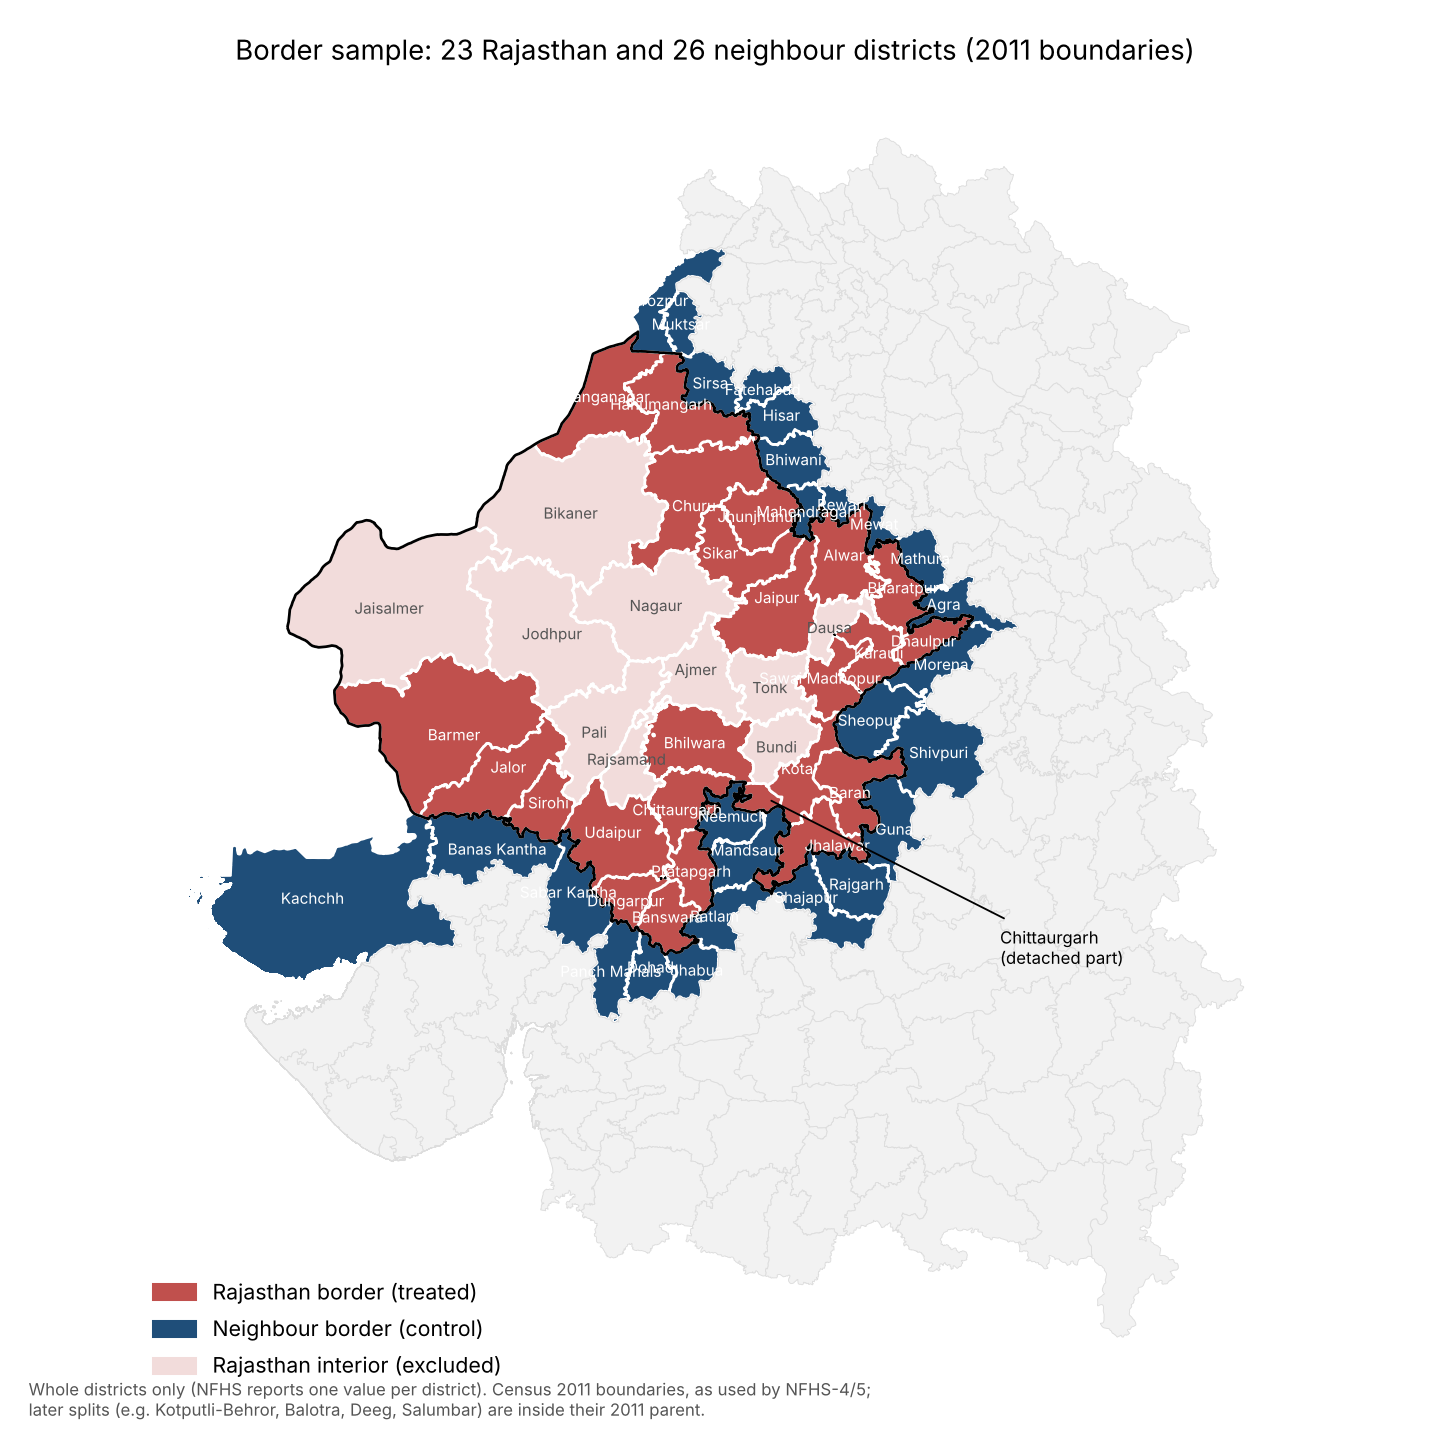
\includegraphics[width=\textwidth,height=0.80\textheight,keepaspectratio,trim=0 95 0 60,clip]{fig_border_map.png}
\end{column}
\begin{column}{0.36\textwidth}
\scriptsize
\textbf{23 Rajasthan $\times$ 26 neighbour districts}\\[3pt]
\textcolor[RGB]{192,80,77}{$\blacksquare$} Rajasthan border (treated)\\
\textcolor[RGB]{31,78,121}{$\blacksquare$} Neighbour border (control)\\
\textcolor[RGB]{242,220,219}{$\blacksquare$} Rajasthan interior (excluded)
\begin{itemize}
\item Districts \textbf{touching} across the state line (2011 map; $\ge$ 7 km shared border)
\item 51 pairs: MP 22, Haryana 13, Gujarat 10, Punjab 3, UP 3
\item \textbf{40 pairs} after dropping split districts
\item Whole districts only
\end{itemize}
\end{column}
\end{columns}
\end{frame}

\begin{frame}[t]{Empirical strategy}
\small
For district $i$ in contiguous pair $p$:
\[
\Delta Y_{ip} = \beta \cdot \mathit{Rajasthan}_i + \gamma_p + \varepsilon_{ip},
\qquad \Delta Y = Y^{\text{NFHS-5}} - Y^{\text{NFHS-4}}
\]
\begin{itemize}
\item $\Delta Y$: differencing removes everything fixed about a district (district FE)
\item $\gamma_p$: pair fixed effect $\Rightarrow$ compare only with the touching neighbour
\item $\beta$: within-pair difference-in-differences
\item SEs \textbf{two-way clustered} by Rajasthan and neighbour district
\end{itemize}
\begin{block}{Identifying assumption}
\textbf{Parallel trends across the border}: without BSBY, both sides would have changed alike. Tested with a three-round state event study.
\end{block}
\scriptsize Robustness: drop Gujarat (own scheme); MP border only; pairs $\ge$ 10 km; control for NFHS-4 level; leave-one-out; OOP capping; placebos.
\end{frame}

%%%%%%%%%%%%%%%%%%%%%%%%%%%%%%%%%%%%%%%%%%%%%%%%%%%%%%%%%%%%%%%%%%%%%%%%%%%%%%%%
\section{Results}

\begin{frame}[t]{Pre-trends: state event study}
\begin{columns}[T]
\begin{column}{0.62\textwidth}
\centering
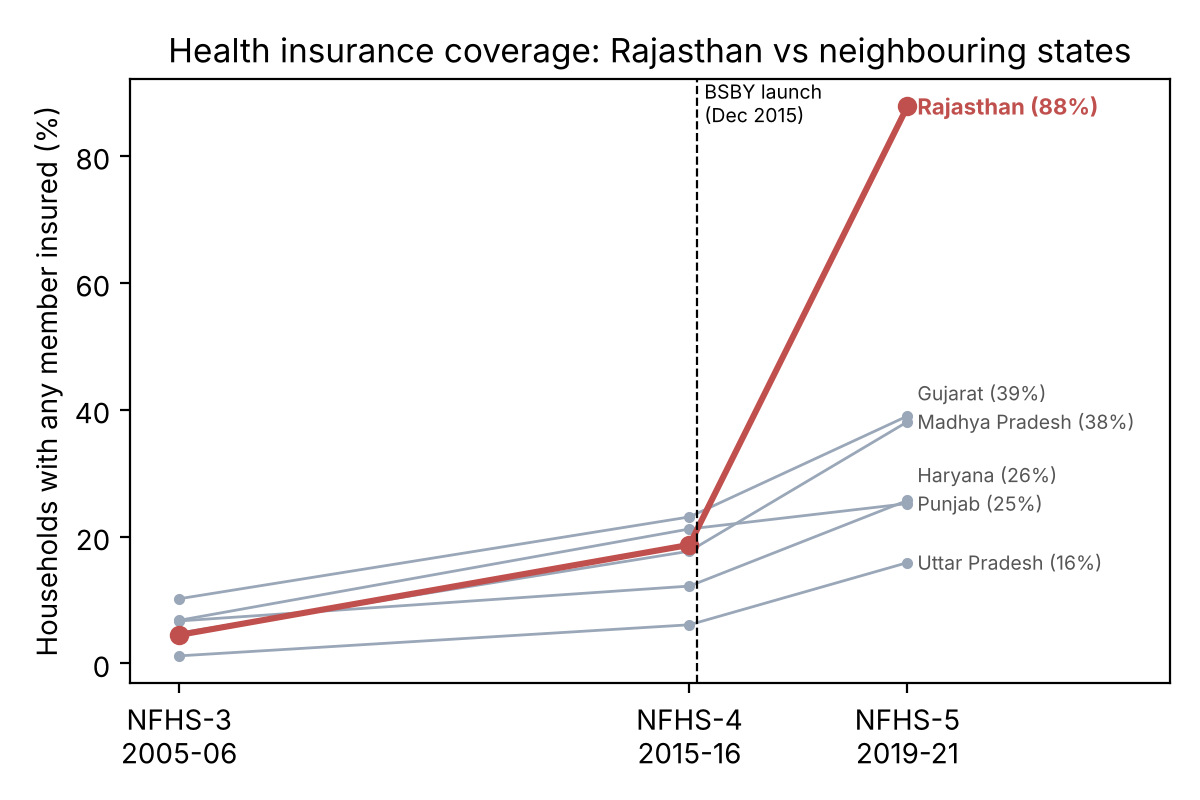
\includegraphics[width=\textwidth]{fig_state_event_study.png}
\end{column}
\begin{column}{0.36\textwidth}
\scriptsize
\begin{itemize}
\item Pre-period DiD $\phi_2 = +4.1$ pp: roughly parallel
\item Post-period DiD $\phi_3 = +56.4$ pp
\item Trend-adjusted: \textbf{+52.3 pp}
\item Permutation: Rajasthan \textbf{1st of 27} states, p = 0.037
\end{itemize}
\end{column}
\end{columns}
\end{frame}

\begin{frame}[t]{Main result: coverage}
\begin{columns}[T]
\begin{column}{0.60\textwidth}
\centering
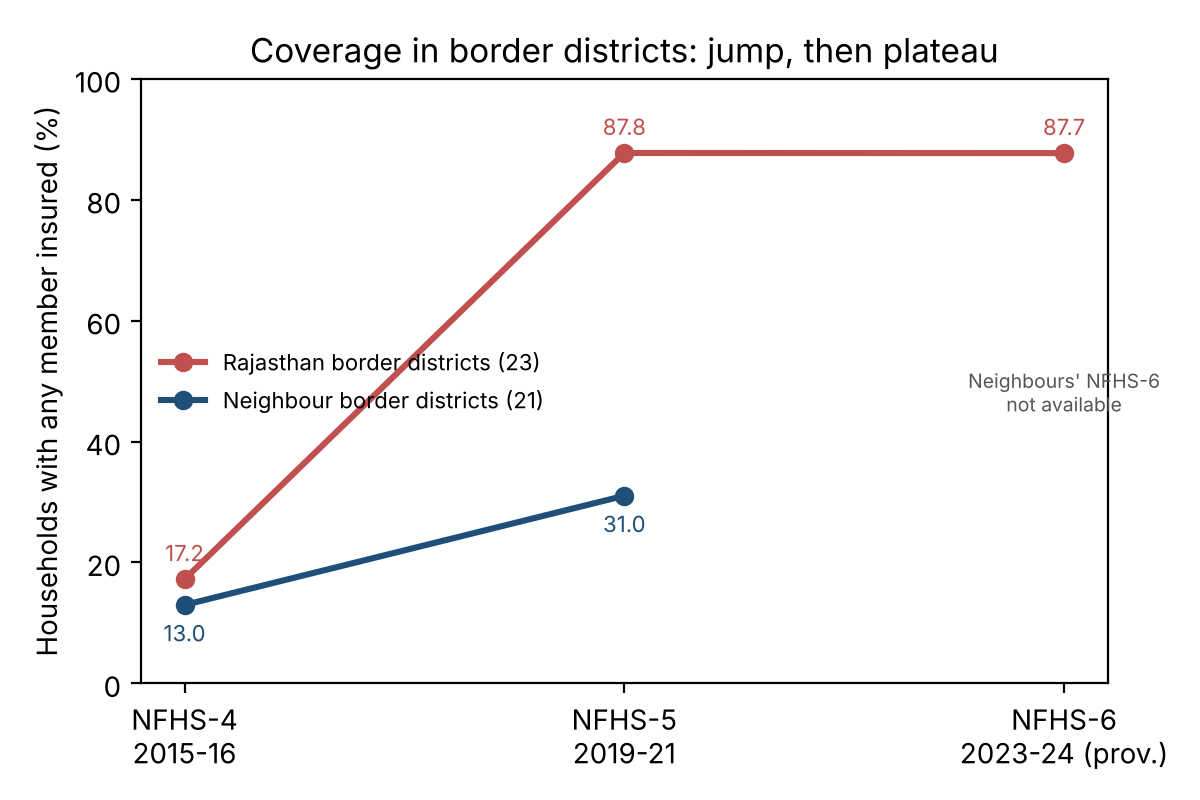
\includegraphics[width=\textwidth]{fig_coverage_three_rounds.png}
\end{column}
\begin{column}{0.38\textwidth}
\scriptsize
\begin{itemize}
\item Rajasthan: 17.2 $\rightarrow$ 87.8 $\rightarrow$ 87.7\%
\item Neighbours: 13.0 $\rightarrow$ 31.0\%
\item Raw DiD: 70.6 $-$ 18.0 = 52.6
\item \hl{Regression: $\beta$ = +52.8 pp (SE 5.1), p $<$ 0.001}
\item Neighbours reach 64.1\% by 2023--24 (next slide)
\end{itemize}
\end{column}
\end{columns}
\end{frame}

\begin{frame}[t]{Did Rajasthan's lead last?}
\small
\textbf{Insurance coverage in border districts (\% of households)}\\[3pt]
\begin{tabular}{@{}lccc@{}}
\toprule
 & \textbf{2015--16} & \textbf{2019--21} & \textbf{2023--24} \\
 & \scriptsize NFHS-4 & \scriptsize NFHS-5 & \scriptsize NFHS-6 \\
\midrule
Rajasthan & 17 & \textbf{88} & \textbf{88} \\
Neighbours & 13 & 31 & \textbf{64} \\
\bottomrule
\end{tabular}

\vspace{5pt}
\begin{itemize}
\item \textbf{2015--21:} BSBY puts Rajasthan 53 pp ahead
\item \textbf{2021--24:} neighbours catch up under PM-JAY
\item \textbf{2023--24:} Rajasthan still \textbf{15 pp} ahead (p = 0.03)
\end{itemize}

\begin{block}{Takeaway}
BSBY gave Rajasthan near-universal coverage \textbf{years before} the national scheme reached its neighbours.
\end{block}

\tiny NFHS-6 provisional (official IIPS compendiums). 15 pp = border-pair estimate excluding 3 Gujarat districts with revised NFHS-5 figures. Placebos flat 2019--24; women's schooling +3.6 pp over 2015--24 (p = 0.04).
\end{frame}

\begin{frame}[t]{All outcomes}
\scriptsize 40 pairs, two-way clustered SEs\par\vspace{4pt}
\scriptsize
\begin{tabular}{@{}lrrrr@{}}
\toprule
\textbf{Outcome} & $\boldsymbol{\beta}$ \textbf{(SE)} & \textbf{p} & \textbf{SD units} & \textbf{+ NFHS-4 level} \\
\midrule
\textbf{Insurance coverage (pp)} & \textbf{+52.8 (5.1)} & \textbf{$<$0.001} & 7.3 & +55.1 (4.2) \\
OOP per delivery (real Rs) & $-$356 (840) & 0.67 & $-$0.44 & +227 (212) \\
log OOP & $-$0.08 (0.31) & 0.80 & $-$0.17 & +0.09 (0.12) \\
Institutional births (pp) & $-$1.2 (2.3) & 0.62 & $-$0.09 & +0.8 (1.3) \\
Public-facility births (pp) & +2.4 (5.4) & 0.66 & 0.12 & +5.5 (3.9) \\
\emph{Placebo:} electricity (pp) & +3.2 (3.5) & 0.35 & 0.56 & $-$0.1 (0.6) \\
\emph{Placebo:} women 10+ yrs school & +3.1 (1.7) & 0.08 & 0.24 & +2.8 (1.5) \\
\bottomrule
\end{tabular}
\vspace{6pt}

\begin{itemize}
\item Coverage: drop Gujarat +51.2; MP only +45.4; pairs $\ge$10 km +52.0; leave-one-district-out +51.3 to +53.9
\item Nothing else significant in any sample; women's-schooling placebo borderline
\end{itemize}
\end{frame}

\begin{frame}[t]{Robustness at a glance}
\centering
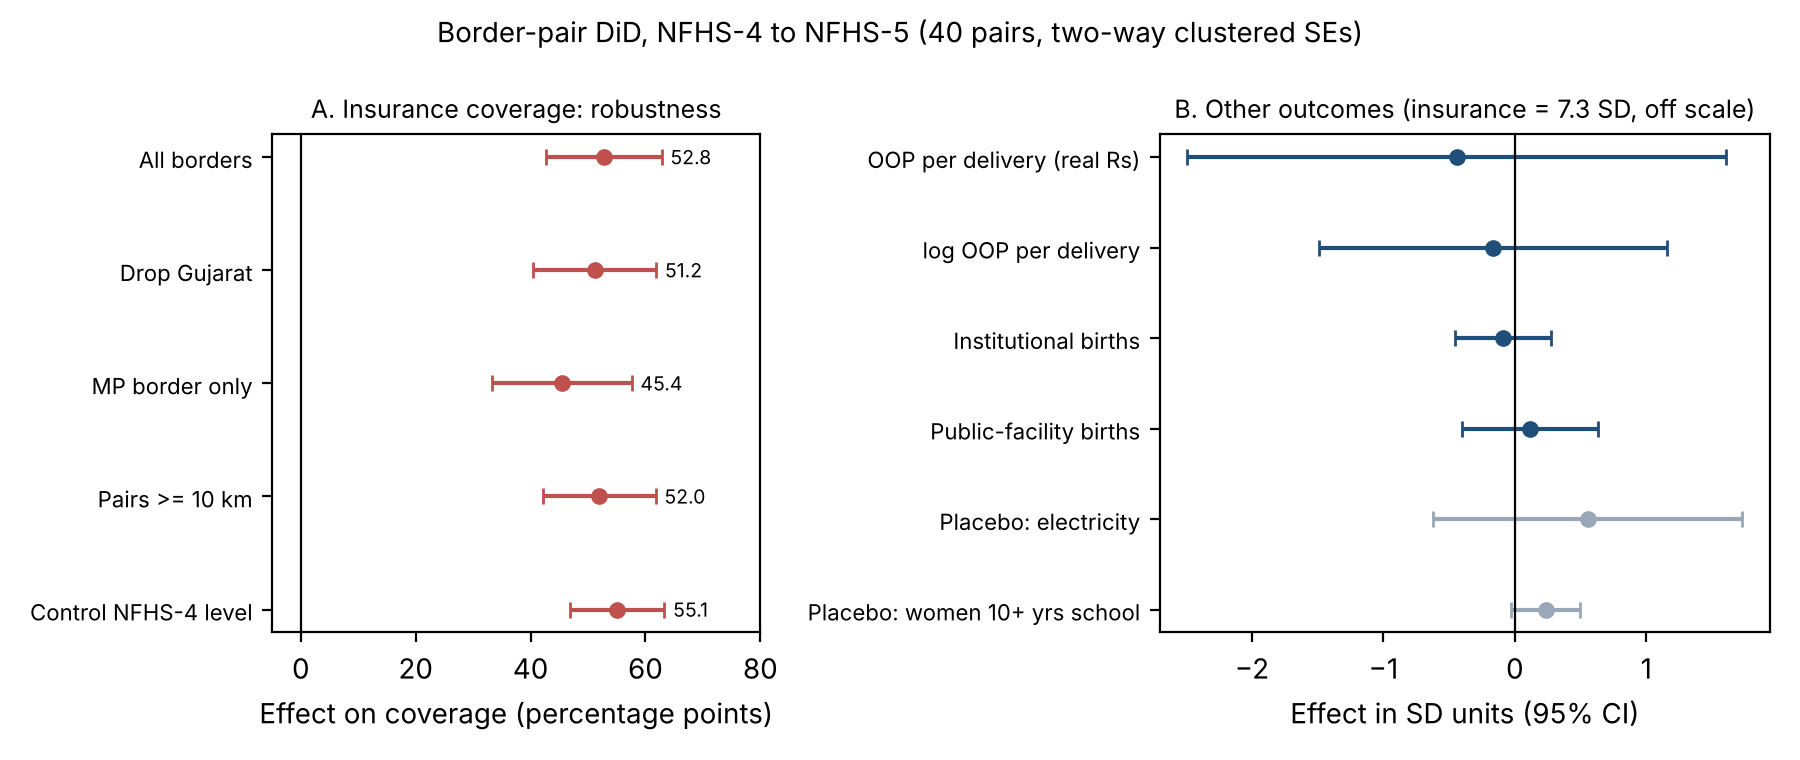
\includegraphics[width=\textwidth]{fig_coefficients.png}
\vspace{2pt}

\scriptsize Panel A: coverage across specifications. Panel B: other outcomes in SD units (95\% CI); grey = placebos.
\end{frame}

\begin{frame}[t]{Out-of-pocket spending}
\small
The estimated effect of BSBY on out-of-pocket spending per delivery is $-$\Rs 356 and is not statistically significant. We interpret this as inconclusive rather than as evidence of no effect, for three reasons.

\vspace{6pt}
\begin{enumerate}
\item \textbf{Low precision.} The 95\% confidence interval ($-$\Rs 2,003 to +\Rs 1,291) is wider than the baseline mean of \Rs 2,235. The minimum detectable effect (\Rs 2,352) exceeds the baseline, so even a complete elimination of delivery costs would probably go undetected.

\item \textbf{Unstable point estimate.} Rajasthan's border districts started with higher spending. Controlling for initial levels reverses the sign (+\Rs 227), and excluding a single district (Baran) gives +\Rs 30.

\item \textbf{Limited relevance of the outcome.} Deliveries in public facilities have been free under JSSK since 2011 in all states. BSBY mainly finances hospitalisations, for which NFHS reports no district-level spending.
\end{enumerate}

\vspace{3pt}
These findings are consistent with Karan, Yip \& Mahal (2017), who report no reduction in out-of-pocket spending under RSBY.
\end{frame}

%%%%%%%%%%%%%%%%%%%%%%%%%%%%%%%%%%%%%%%%%%%%%%%%%%%%%%%%%%%%%%%%%%%%%%%%%%%%%%%%
\section{Cost-effectiveness}

\begin{frame}[t]{Cost-effectiveness}
\scriptsize
\begin{columns}[T]
\begin{column}{0.55\textwidth}
\centering
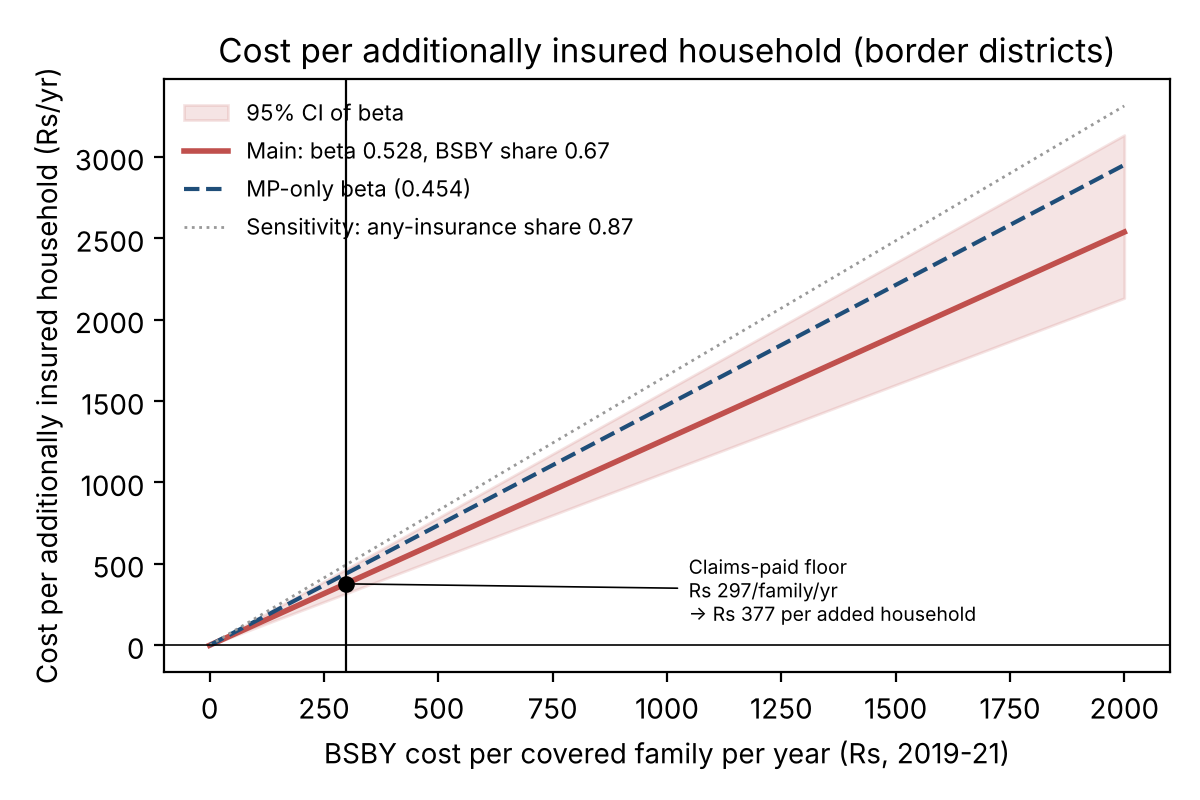
\includegraphics[width=\textwidth]{fig_cost_effectiveness.png}
\end{column}
\begin{column}{0.43\textwidth}
\[
\frac{\text{cost/family} \times s_{BSBY} - p_{RSBY}\,c_{cf}}{\beta}
\]
\begin{itemize}
\item Cost/family = \textbf{\Rs 297}/yr: claims paid (\Rs 295.63 cr, 1.16 yrs, 1 crore families), a \emph{floor} on the premium
\item $s_{BSBY} = 0.67$ (SIHFW p.\ 17)
\item $p_{RSBY} = 0$ (early rollout, Karan p.\ 84)
\end{itemize}
\end{column}
\end{columns}
\vspace{2pt}
\begin{block}{Result (incremental cost-effectiveness ratio; Dhaliwal et al.\ 2013)}
At least \textbf{\Rs 377} per additionally insured household per year (CI of $\beta$: \Rs 317--466; MP-only: \Rs 439), measured against the 2019--21 gap. \textbf{Break-even:} each such household must gain $\ge$ \Rs 377/yr. As neighbours catch up, the cost per unit of \emph{lasting} advantage rises.
\end{block}
\end{frame}

%%%%%%%%%%%%%%%%%%%%%%%%%%%%%%%%%%%%%%%%%%%%%%%%%%%%%%%%%%%%%%%%%%%%%%%%%%%%%%%%
\section{Conclusions}

\begin{frame}[t]{Discussion}
\small
\begin{itemize}
\item \textbf{Coverage:} border estimate (+52.8) and trend-adjusted state estimate (+52.3) agree; by 2023--24 PM-JAY narrowed the gap to $\sim$15 pp, so BSBY's gain was mainly \emph{timing}.
\item \textbf{Financial protection:} our OOP null agrees with RSBY evidence (Karan et al.) and does not contradict Karnataka's tertiary-care gains (Sood et al.): we measure a margin insurance barely touches, at district resolution.
\item \textbf{Who benefits:} Dupas \& Jain find women use BSBY less; household coverage cannot see this.
\item \textbf{Value for money:} $\ge$ \Rs 377 per additionally insured household; $\sim$40\% of spending reaches households that had some insurance anyway.
\end{itemize}
\end{frame}

\begin{frame}[t]{Conclusions}
\begin{enumerate}
\item \textbf{BSBY worked as a coverage policy, and worked early:} +53 pp relative to the border by 2019--21, robust to every check; neighbours caught up to within 15 pp by 2023--24.
\item \textbf{Financial protection is unproven, not disproven:} OOP per delivery is the wrong margin and the design is underpowered for it.
\item \textbf{Cost:} at least \Rs 377 per additionally insured household per year (against the 2019--21 gap); benefits must exceed this to justify it.
\item \textbf{Policy:} a state scheme can deliver near-universal coverage years before the national scheme does; evaluations should measure hospitalisation spending and health, not just enrolment.
\end{enumerate}
\end{frame}

\begin{frame}[t]{Limitations and future work}
\footnotesize
\begin{columns}[T]
\begin{column}{0.5\textwidth}
\textbf{Limitations}
\begin{itemize}
\item NFHS-4 baseline began 6 weeks after launch $\Rightarrow$ $\beta$ is a lower bound
\item Scheme vs scheme, not insurance vs none
\item District averages; large districts
\item OOP: deliveries only, underpowered
\item One pre-period, state level
\item Cost is a claims floor; benefits not monetised
\item NFHS-6 provisional; Gujarat NFHS-5 insurance revised
\item Long-difference schooling placebo significant (p = 0.04)
\end{itemize}
\end{column}
\begin{column}{0.48\textwidth}
\textbf{Future work}
\begin{itemize}
\item NSS 71st vs 75th: OOP per hospitalisation
\item NFHS GPS clusters: spatial RD (Dell 2010; Sood et al.\ 2014)
\item Link neighbours' catch-up to PM-JAY rollout
\item Actual premium $\Rightarrow$ MVPF / value of risk protection
\end{itemize}
\end{column}
\end{columns}
\end{frame}

%%%%%%%%%%%%%%%%%%%%%%%%%%%%%%%%%%%%%%%%%%%%%%%%%%%%%%%%%%%%%%%%%%%%%%%%%%%%%%%%
\section*{References}

\begin{frame}[t]{References}
\tiny
\begin{itemize}
\item Abadie, A., Diamond, A., \& Hainmueller, J. (2010). Synthetic control methods for comparative case studies. \emph{JASA}, 105(490), 493--505.
\item Card, D., \& Krueger, A. B. (1994). Minimum wages and employment. \emph{American Economic Review}, 84(4), 772--793.
\item Conley, T. G., \& Taber, C. R. (2011). Inference with ``difference in differences'' with a small number of policy changes. \emph{REStat}, 93(1), 113--125.
\item Dell, M. (2010). The persistent effects of Peru's mining mita. \emph{Econometrica}, 78(6), 1863--1903.
\item Dhaliwal, I., Duflo, E., Glennerster, R., \& Tulloch, C. (2013). Comparative cost-effectiveness analysis to inform policy in developing countries. J-PAL.
\item Dube, A., Lester, T. W., \& Reich, M. (2010). Minimum wage effects across state borders. \emph{REStat}, 92(4), 945--964.
\item Dupas, P., \& Jain, R. (2021, rev.\ 2023). Women left behind: Gender disparities in utilization of government health insurance in India. NBER WP 28972.
\item Finkelstein, A., \& McKnight, R. (2008). What did Medicare do? \emph{Journal of Public Economics}, 92(7), 1644--1668.
\item Hendren, N., \& Sprung-Keyser, B. (2020). A unified welfare analysis of government policies. \emph{QJE}, 135(3), 1209--1318.
\item IIPS. National Family Health Survey (NFHS-3, 4, 5) fact sheets; NFHS-6 state compendiums: Rajasthan, Gujarat, Haryana, MP, Punjab, UP (provisional, 2026).
\item Karan, A., Yip, W., \& Mahal, A. (2017). Extending health insurance to the poor in India: RSBY and out of pocket spending. \emph{Social Science \& Medicine}, 181, 83--92.
\item Kling, J. R., Liebman, J. B., \& Katz, L. F. (2007). Experimental analysis of neighborhood effects. \emph{Econometrica}, 75(1), 83--119.
\item Patra, N. K. (2026). NFHS-6 provisional district-level data (India): independent compilation. GitHub (cross-check).
\item SIHFW Rajasthan. \emph{Bhamashah Swasthya Bima Yojana} (presentation). Jaipur.
\item Sood, N., et al.\ (2014). Government health insurance for people below poverty line in India. \emph{BMJ}, 349, g5114.
\end{itemize}
\end{frame}

{\usebackgroundtemplate{
\includegraphics[width=\paperwidth,height=\paperheight]{white_bg.png}}
\begin{frame}[plain,c]
\begin{center}
{\color{IITRBlue}\LARGE \underline{Thank you.}}\\[1.5em]
\small Code, data and full explainer:\\
\url{https://github.com/ipsanmoljj/india-welfare-analysis}
\end{center}
\end{frame}
}

\end{document}
